\begin{figure*}[ht]
\begin{subfigure}{.5\textwidth}
  \centering
  % include third image
  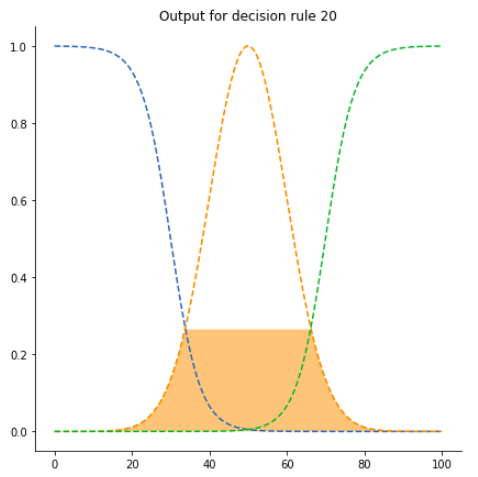
\includegraphics[width=.8\linewidth]{figures/third/min1.png}  
  \caption{Output for decision rule 20 with the T-norm minimum.}
  \label{fig:3min1}
\end{subfigure}
\begin{subfigure}{.5\textwidth}
  \centering
  % include third image
  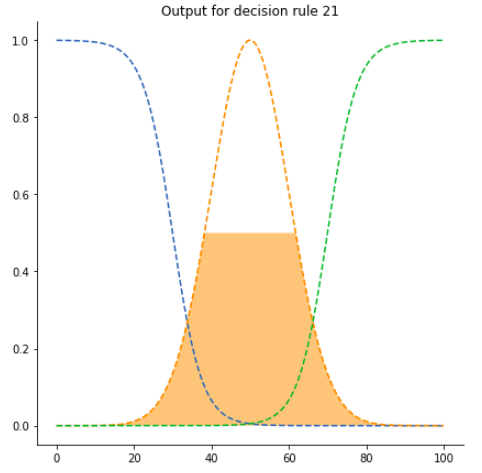
\includegraphics[width=.8\linewidth]{figures/third/min2.png}  
  \caption{Output for decision rule 21 with the T-norm minimum.}
  \label{fig:3min2}
\end{subfigure}
\begin{subfigure}{.5\textwidth}
  \centering
  % include third image
  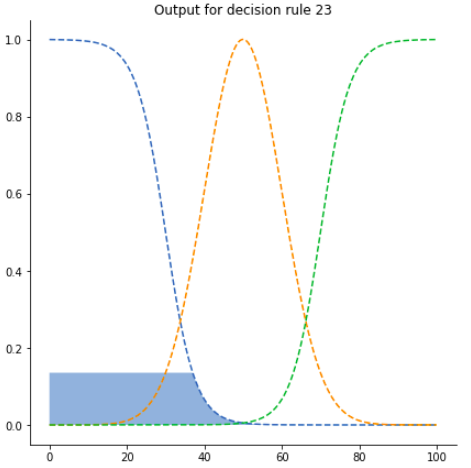
\includegraphics[width=.8\linewidth]{figures/third/min3.png}  
  \caption{Output for decision rule 23 with the T-norm minimum.}
  \label{fig:3min3}
\end{subfigure}
\begin{subfigure}{.5\textwidth}
  \centering
  % include third image
  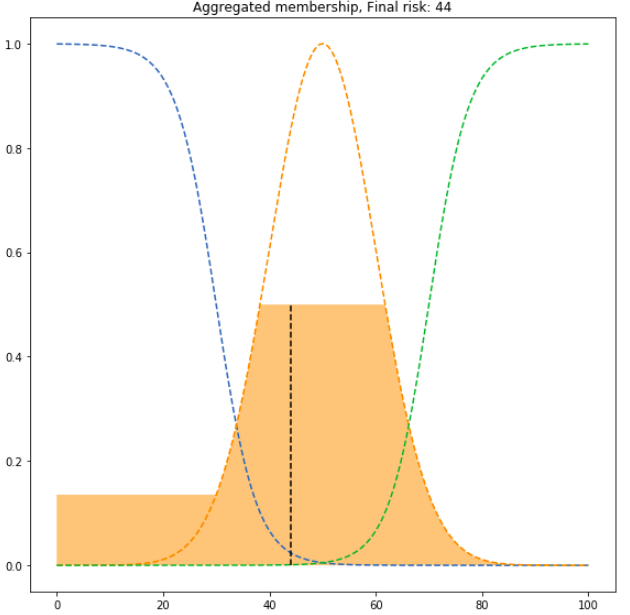
\includegraphics[width=.8\linewidth]{figures/third/min-centroid.png}  
  \caption{Final aggregation result with the centroid method for defuzzification.}
  \label{fig:3min-centroid}
\end{subfigure}
\begin{subfigure}{.5\textwidth}
  \centering
  % include third image
  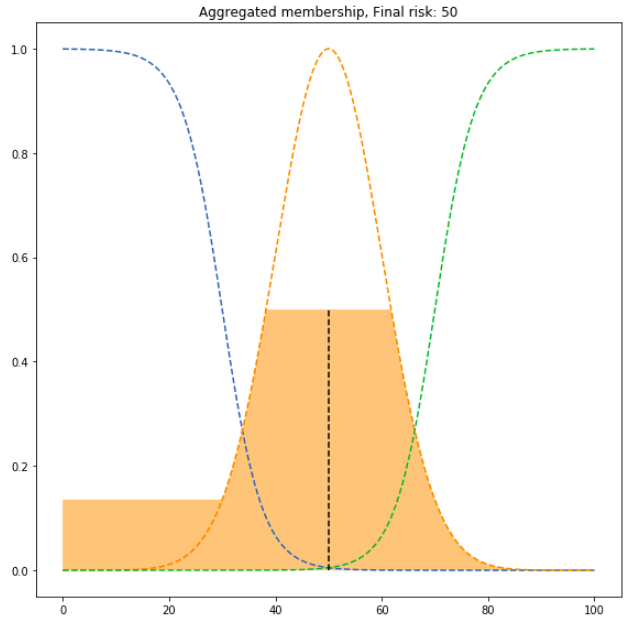
\includegraphics[width=.8\linewidth]{figures/third/min-mom.png}  
  \caption{Final aggregation result with the mean of maximum method for defuzzification.}
  \label{fig:3min-mom}
\end{subfigure}
\begin{subfigure}{.5\textwidth}
  \centering
  % include third image
  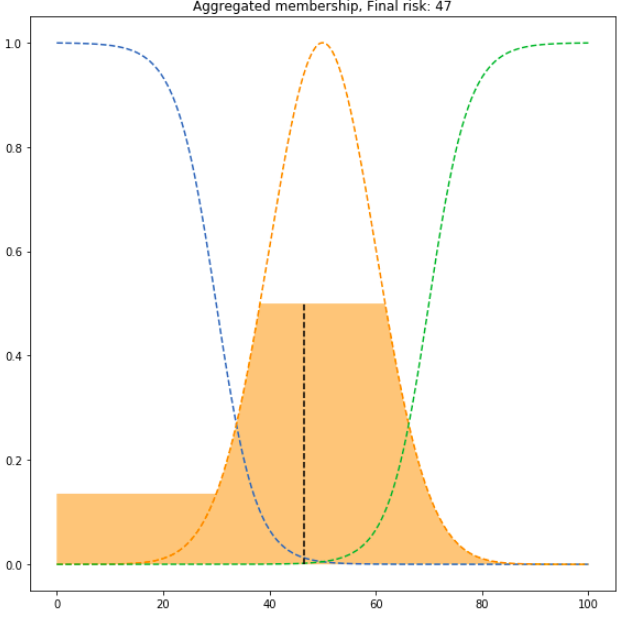
\includegraphics[width=.8\linewidth]{figures/third/min-bisector.png}  
  \caption{Final aggregation result with the bisector method for defuzzification.}
  \label{fig:3min-bisector}
\end{subfigure}
\caption{Results for test case 3 using the T-norm minimum.}
\label{fig:testcase3min}
\end{figure*}

\begin{figure*}[ht]
\begin{subfigure}{.5\textwidth}
  \centering
  % include third image
  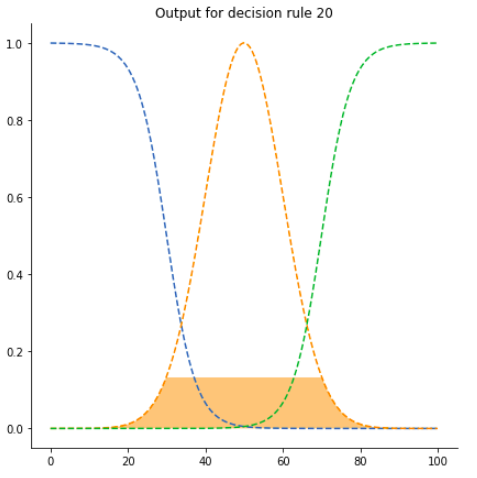
\includegraphics[width=.8\linewidth]{figures/third/prod1.png}  
  \caption{Output for decision rule 20 with the T-norm product.}
  \label{fig:3prod1}
\end{subfigure}
\begin{subfigure}{.5\textwidth}
  \centering
  % include third image
  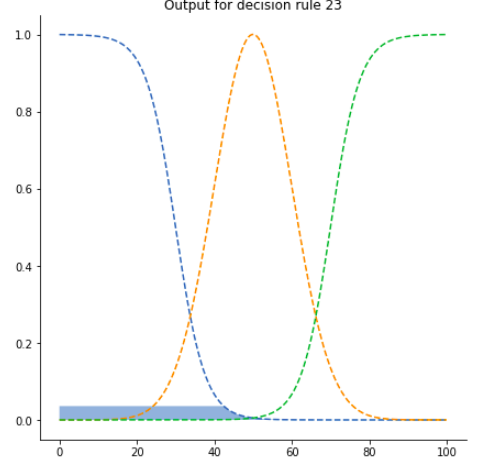
\includegraphics[width=.8\linewidth]{figures/third/prod2.png}  
  \caption{Output for decision rule 23 with the T-norm product.}
  \label{fig:3prod2}
\end{subfigure}
\begin{subfigure}{.5\textwidth}
  \centering
  % include third image
  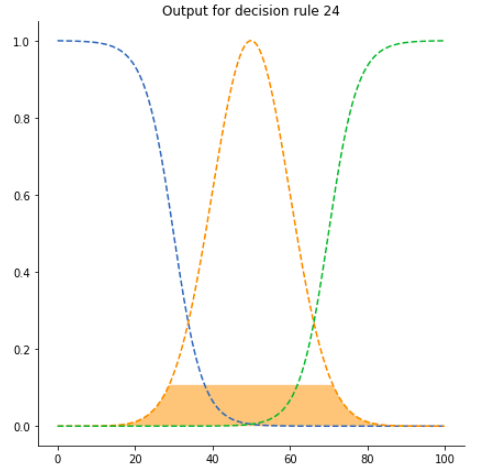
\includegraphics[width=.8\linewidth]{figures/third/prod3.png}  
  \caption{Output for decision rule 24 with the T-norm product.}
  \label{fig:3prod3}
\end{subfigure}
\begin{subfigure}{.5\textwidth}
  \centering
  % include third image
  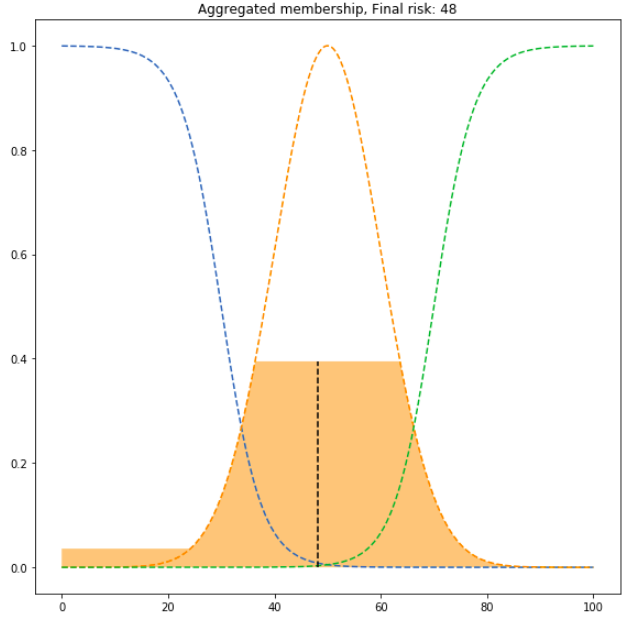
\includegraphics[width=.8\linewidth]{figures/third/prod-centroid.png}  
  \caption{Final aggregation result with the centroid method for defuzzification.}
  \label{fig:3prod-centroid}
\end{subfigure}
\begin{subfigure}{.5\textwidth}
  \centering
  % include third image
  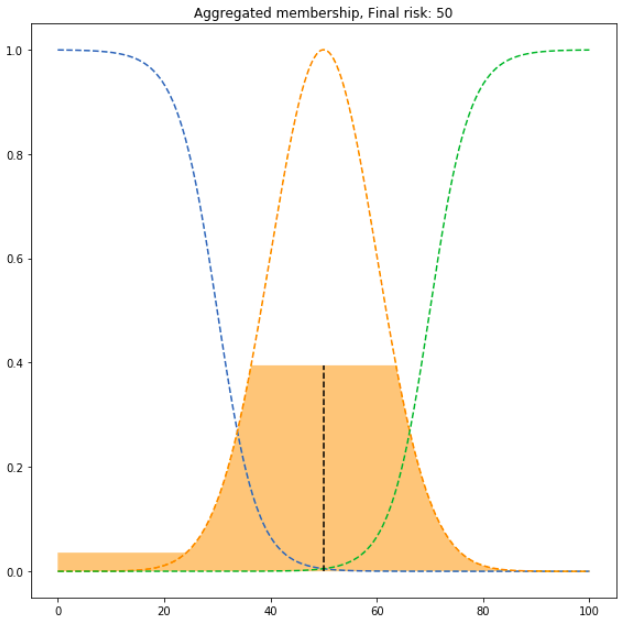
\includegraphics[width=.8\linewidth]{figures/third/prod-mom.png}  
  \caption{Final aggregation result with the mean of maximum method for defuzzification.}
  \label{fig:3prod-mom}
\end{subfigure}
\begin{subfigure}{.5\textwidth}
  \centering
  % include third image
  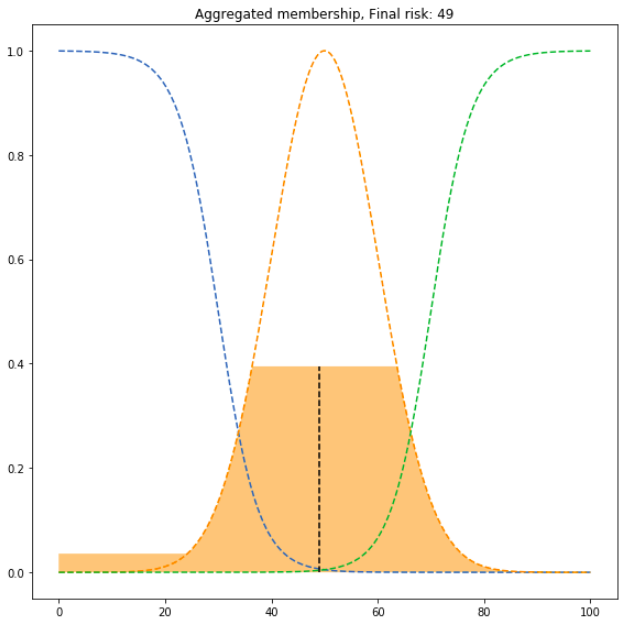
\includegraphics[width=.8\linewidth]{figures/third/prod-bisector.png}  
  \caption{Final aggregation result with the bisector method for defuzzification.}
  \label{fig:3prod-bisector}
\end{subfigure}
\caption{Results for test case 3 using the T-norm product.}
\label{fig:testcase3prod}
\end{figure*}
